\documentclass[12pt,a4paper]{article}
\usepackage[utf8]{inputenc}
\usepackage[T1]{fontenc}
\usepackage[brazil]{babel}
\usepackage{geometry}
\geometry{a4paper, margin=2.5cm}
\usepackage{graphicx}
\usepackage{booktabs}
\usepackage{amsmath}
\usepackage{amssymb}
\usepackage{float}
\usepackage{caption}
\usepackage{xcolor}
\usepackage{listings}
\usepackage{hyperref}
\hypersetup{hidelinks}

\definecolor{codegray}{rgb}{0.5,0.5,0.5}
\definecolor{codegreen}{rgb}{0,0.5,0}
\definecolor{codepurple}{rgb}{0.58,0,0.82}
\definecolor{backcolour}{rgb}{0.96,0.96,0.96}

\lstset{
  backgroundcolor=\color{backcolour},
  commentstyle=\color{codegreen},
  keywordstyle=\color{blue},
  stringstyle=\color{codepurple},
  basicstyle=\ttfamily\scriptsize,
  breakatwhitespace=false,
  breaklines=true,
  captionpos=b,
  keepspaces=true,
  numbers=left,
  numbersep=5pt,
  numberstyle=\tiny\color{codegray},
  showspaces=false,
  showstringspaces=false,
  showtabs=false,
  tabsize=2,
  frame=single,
  language=Python,
  inputencoding=utf8,
  extendedchars=true,
  literate=%
    {á}{{\'a}}1 {é}{{\'e}}1 {í}{{\'i}}1 {ó}{{\'o}}1 {ú}{{\'u}}1
    {Á}{{\'A}}1 {É}{{\'E}}1 {Í}{{\'I}}1 {Ó}{{\'O}}1 {Ú}{{\'U}}1
    {à}{{\`a}}1 {â}{{\^a}}1 {ê}{{\^e}}1 {ô}{{\^o}}1 {î}{{\^i}}1
    {ã}{{\~a}}1 {õ}{{\~o}}1 {ç}{{\c c}}1 {Ç}{{\c C}}1
    {º}{{\textordmasculine}}1 {ª}{{\textordfeminine}}1
}

\begin{document}
\begin{center}
  {\large \textbf{Optativa III --- Redes Neurais Artificiais}}\\[3pt]
  \textbf{Engenharia da Computação --- UEMG Divinópolis}\\[3pt]
  \textbf{Prof. Arismar Morais Gonçalves Júnior} \hfill \textbf{Valor: 12 pontos}\\[10pt]
  {\Large \textbf{5\textsuperscript{o} Projeto Prático --- Rede RBF no Reconhecimento de Padrões}}\\[10pt]
\end{center}
\noindent\textbf{Autor:} Nome do Aluno \hfill \textbf{Data de geração:} 23/06/2026 23:19\\[4pt]
\noindent\rule{\textwidth}{0.4pt}

\section*{Introdução}
A presente implementação treina uma Rede de Função de Base Radial (RBF) para a
detecção da presença de radiação em substâncias nucleares, a partir de 40 condições
conhecidas descritas por duas variáveis características ($x_1$ e $x_2$). A saída
desejada assume $d = +1$ para radiação \textbf{existente} e $d = -1$ para radiação
\textbf{inexistente}. A rede possui duas entradas, dois neurônios ocultos com ativação
gaussiana (base radial) e um neurônio de saída com ativação linear. O treinamento
ocorre em dois estágios: (i) posicionamento dos centros das gaussianas pelo algoritmo
\textit{k-means} (não supervisionado) e (ii) ajuste dos pesos da camada de saída pela
regra Delta generalizada (supervisionado).

\section*{Etapa 1 --- Treinamento da camada escondida (\textit{k-means})}
O treinamento da camada intermediária foi realizado pelo algoritmo \textit{k-means}
com $k = 2$, considerando \textbf{apenas} os padrões com presença de radiação
($d = +1$). Os vetores de pesos (centros) foram inicializados com as duas primeiras
amostras desse subconjunto e atualizados iterativamente até não haver mudança nos
agrupamentos. A variância de cada gaussiana foi obtida pelo critério da distância
quadrática média. A Tabela~\ref{tab:clusters} apresenta os centros e variâncias obtidos.

\begin{table}[H]
\centering
\caption{Clusters do treinamento da camada escondida da rede RBF.}
\label{tab:clusters}
\begin{tabular}{ccccc}
\toprule
\textbf{Cluster} & \textbf{Center ($x_1$)} & \textbf{Center ($x_2$)} & \textbf{Variance} & \textbf{N\textsuperscript{o} padrões} \\
\midrule
1 & 0.164833 & 0.612117 & 0.059611 & 6 \\
2 & 0.398969 & 0.157131 & 0.076920 & 13 \\
\bottomrule
\end{tabular}
\end{table}

\begin{figure}[H]
\centering
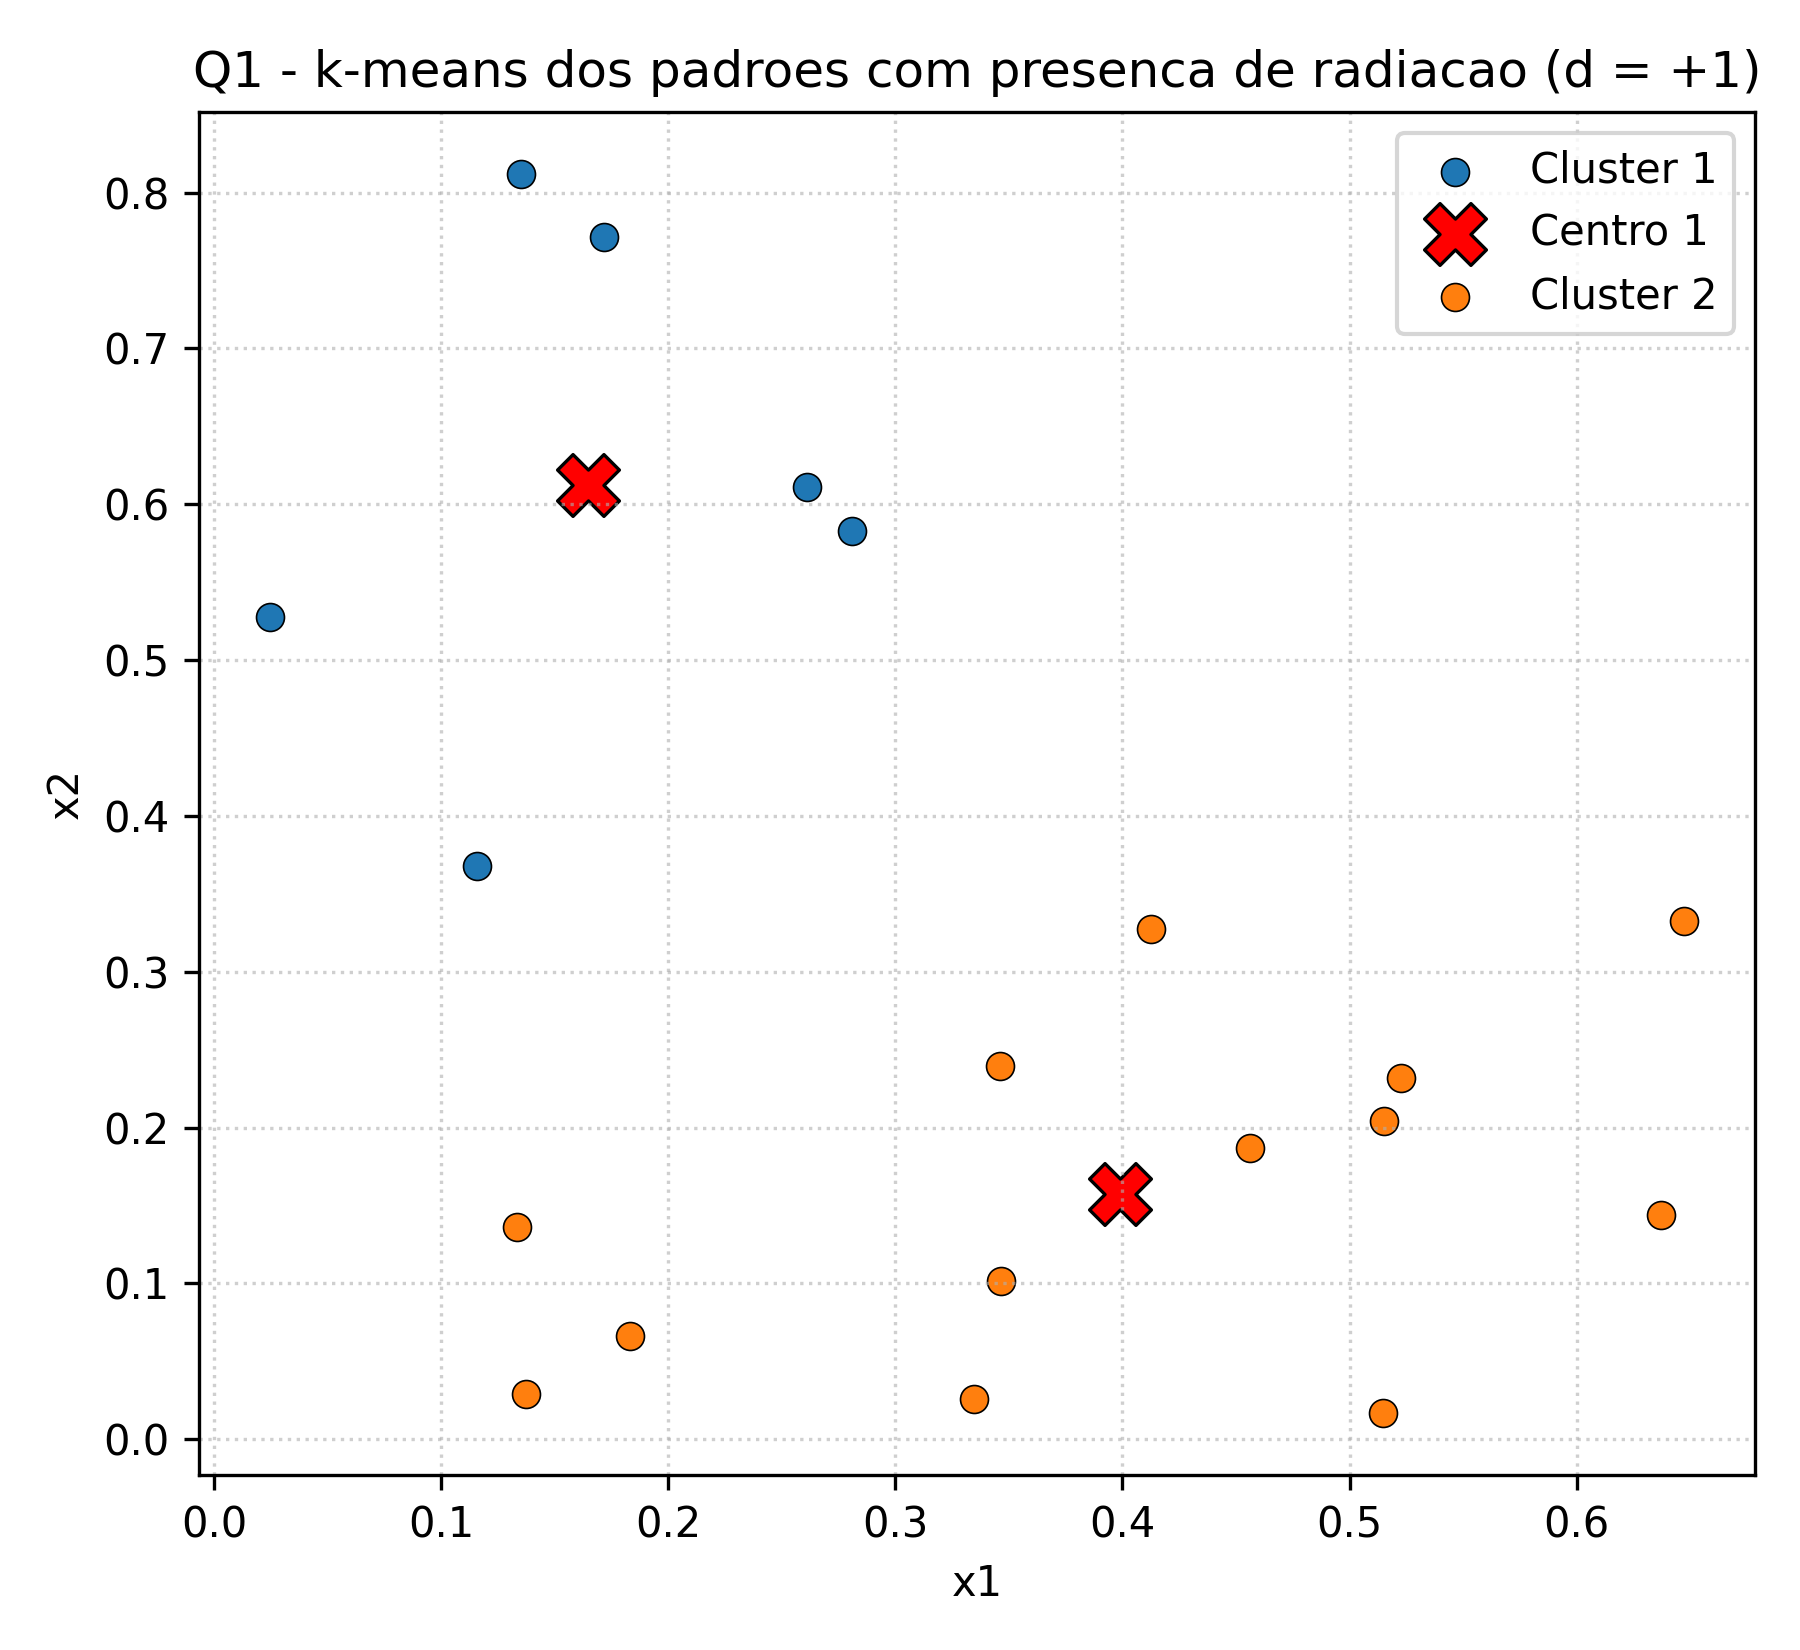
\includegraphics[width=0.68\textwidth]{graphics/q1_clusters_kmeans.png}
\caption{Agrupamentos \textit{k-means} dos padrões com presença de radiação ($d=+1$) e respectivos centros.}
\end{figure}

\section*{Etapa 2 --- Treinamento da camada de saída (regra Delta generalizada)}
O segundo estágio ajustou os pesos do neurônio de saída (ativação linear) pela regra
Delta generalizada, apresentando as amostras individualmente, com taxa de aprendizagem
$\eta = 0.01$ e precisão $\epsilon = 10^{-7}$. 
O treinamento convergiu em \textbf{239} épocas. A Tabela~\ref{tab:pesos} apresenta os pesos finais.

\begin{table}[H]
\centering
\caption{Resultados do segundo estágio de treinamento da rede RBF.}
\label{tab:pesos}
\begin{tabular}{cc}
\toprule
\textbf{Parameter} & \textbf{Value} \\
\midrule
$W^{(2)}_{1,1}$ & 1.597049 \\
$W^{(2)}_{2,1}$ & 2.503513 \\
$\theta_1$ & 1.295083 \\
\bottomrule
\end{tabular}
\end{table}

\section*{Etapa 3 --- Erro quadrático médio por época}
A figura a seguir apresenta a evolução do erro quadrático médio (EQM) em função de
cada época do segundo estágio de treinamento.
O EQM inicial foi de 0.606281 e o final de 0.120814, correspondendo a uma redução de 80.07\% ao longo de 239 épocas.

\begin{figure}[H]
\centering
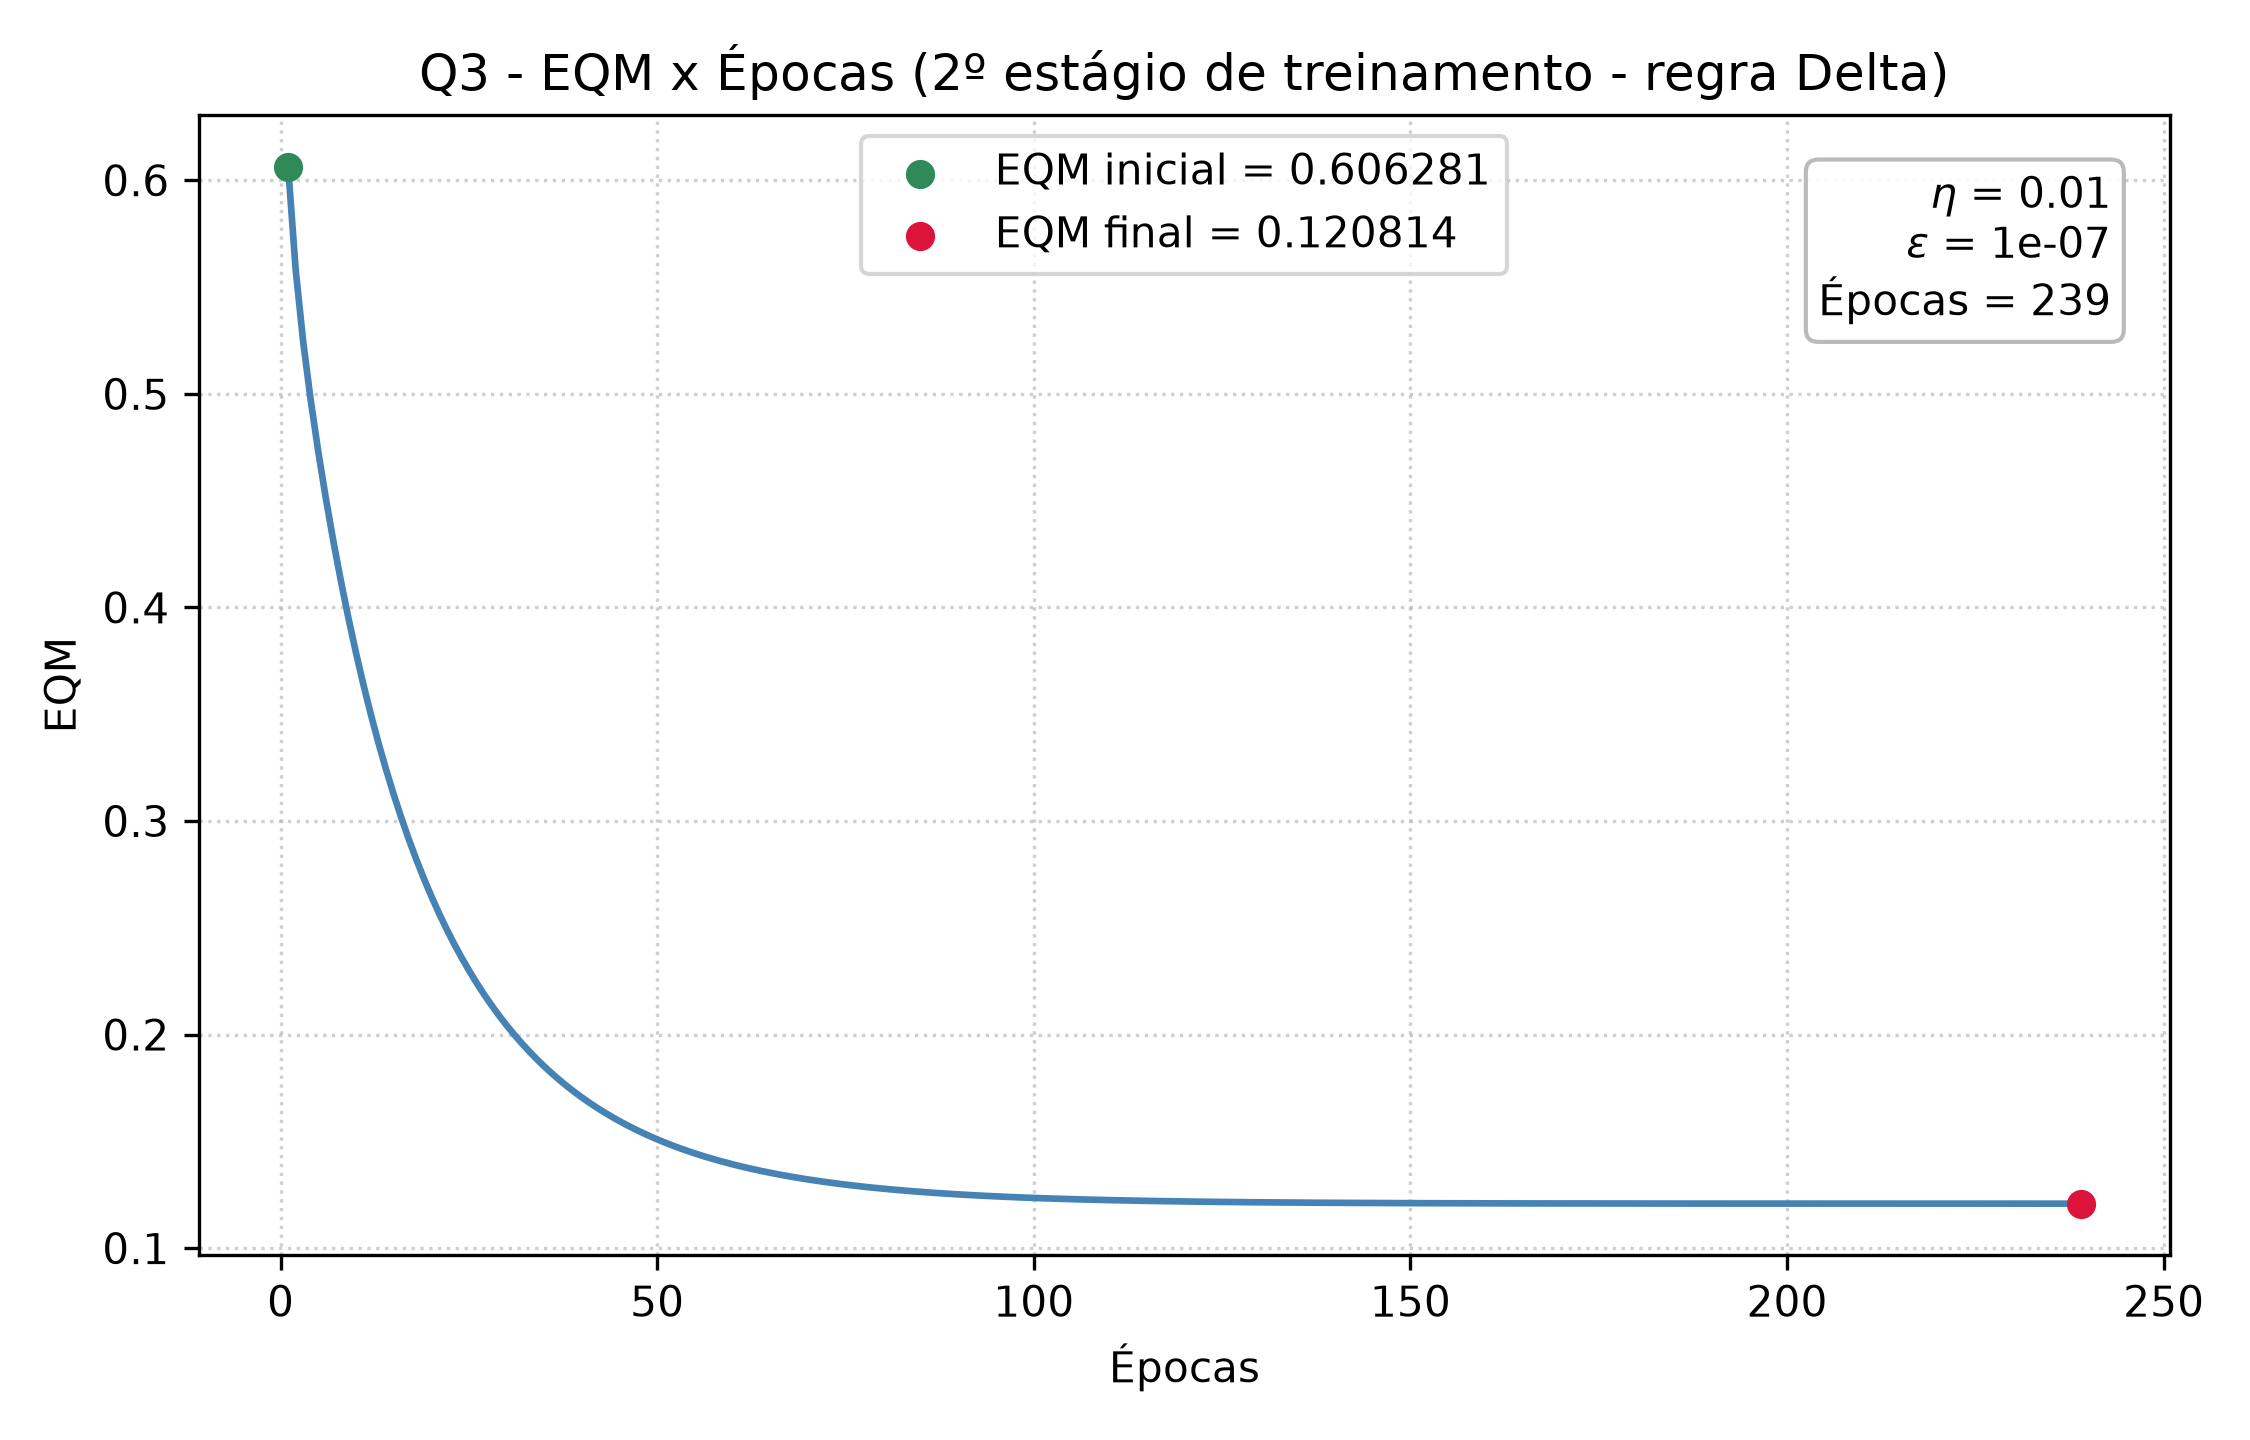
\includegraphics[width=0.82\textwidth]{graphics/q3_eqm_etapa2.png}
\caption{Erro quadrático médio (EQM) em função das épocas do 2\textsuperscript{o} estágio de treinamento.}
\end{figure}

\section*{Etapa 4 --- Validação da rede RBF}
Com os dados de validação e aplicando o pós-processamento ($y_{pos} = 1$ se
$y \geq 0$ e $y_{pos} = -1$ se $y < 0$), obtiveram-se os resultados da
Tabela~\ref{tab:validacao}.

\begin{table}[H]
\centering
\caption{Resultados da validação da rede RBF.}
\label{tab:validacao}
\begin{tabular}{cccccc}
\toprule
\textbf{Sample} & $x_1$ & $x_2$ & $d$ & $y$ & $y^{post}$ \\
\midrule
1 & 0.8705 & 0.9329 & -1 & -1.2729 & -1 \\
2 & 0.0388 & 0.2703 & 1 & 0.2208 & 1 \\
3 & 0.8236 & 0.4458 & -1 & -0.8107 & -1 \\
4 & 0.7075 & 0.1502 & 1 & 0.0755 & 1 \\
5 & 0.9587 & 0.8663 & -1 & -1.2780 & -1 \\
6 & 0.6115 & 0.9365 & -1 & -1.1351 & -1 \\
7 & 0.3534 & 0.3646 & 1 & 1.2810 & 1 \\
8 & 0.3268 & 0.2766 & 1 & 1.4092 & 1 \\
9 & 0.6129 & 0.4518 & -1 & 0.0013 & 1 \\
10 & 0.9948 & 0.4962 & -1 & -1.1727 & -1 \\
\midrule
\multicolumn{5}{r}{\textbf{Success rate (\%)}} & \textbf{90.00} \\
\bottomrule
\end{tabular}
\end{table}
A rede classificou corretamente 9 de 10 amostras de validação.

\section*{Etapa 5 --- Matriz de confusão e parâmetros}
Considerando como classe positiva a presença de radiação ($+1$), a matriz de confusão
obtida na validação é apresentada na Tabela~\ref{tab:confusao} e os parâmetros de
classificação na Tabela~\ref{tab:metricas}.

\begin{table}[H]
\centering
\caption{Matriz de confusão (linha = classe verdadeira, coluna = classe predita).}
\label{tab:confusao}
\begin{tabular}{ccc}
\toprule
 & \textbf{Predito $+1$} & \textbf{Predito $-1$} \\
\midrule
\textbf{Real $+1$} & 4 & 0 \\
\textbf{Real $-1$} & 1 & 5 \\
\bottomrule
\end{tabular}
\end{table}

\begin{table}[H]
\centering
\caption{Parâmetros de classificação da rede RBF.}
\label{tab:metricas}
\begin{tabular}{lc}
\toprule
\textbf{Parâmetro} & \textbf{Valor} \\
\midrule
N\textsuperscript{o} de acertos (Nacertos) & 9 \\
N\textsuperscript{o} de erros (Nerros) & 1 \\
Acurácia & 90.00\% \\
Sensibilidade & 100.00\% \\
Especificidade & 83.33\% \\
Precisão & 80.00\% \\
\bottomrule
\end{tabular}
\end{table}

\begin{figure}[H]
\centering
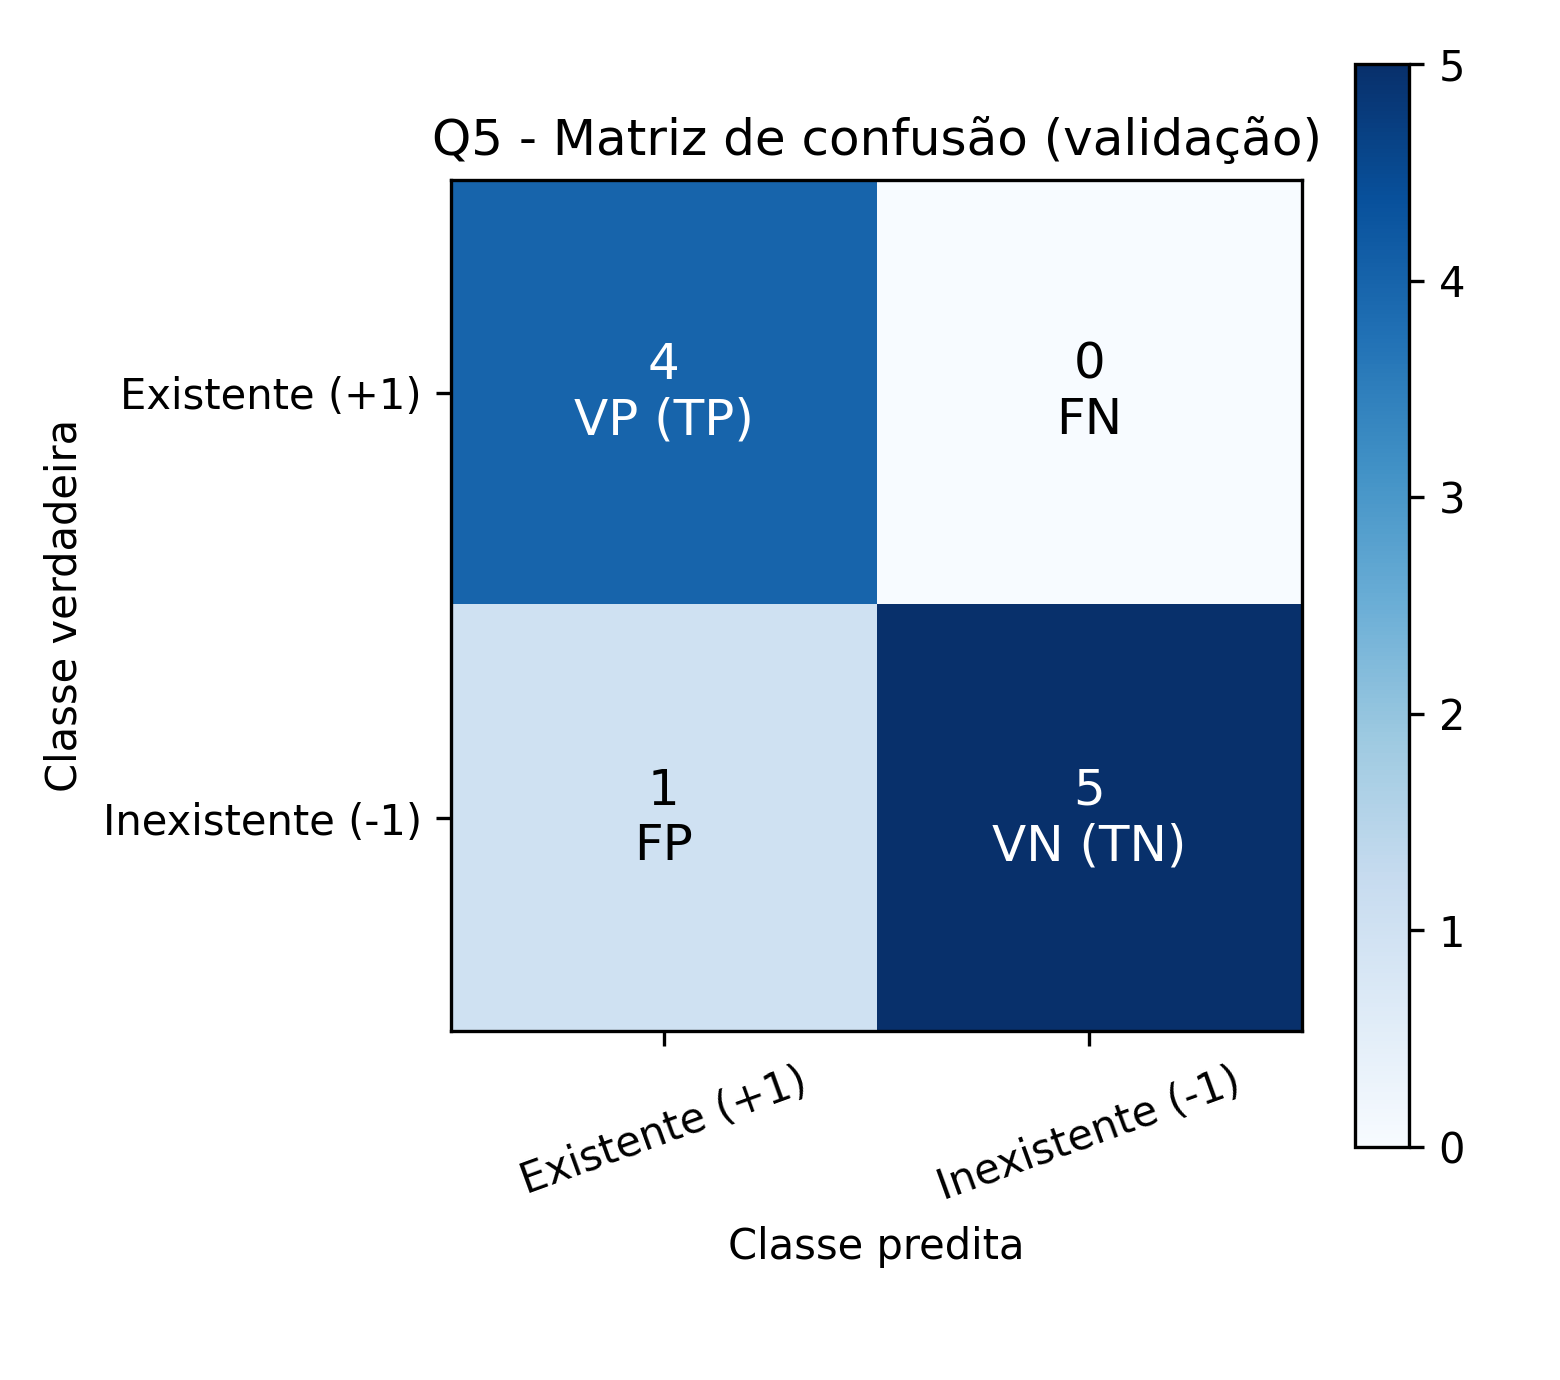
\includegraphics[width=0.58\textwidth]{graphics/q5_matriz_confusao.png}
\caption{Matriz de confusão da validação da rede RBF.}
\end{figure}

\subsection*{Estratégias para melhoria do desempenho}
Caso seja necessário melhorar o desempenho da rede, podem ser adotadas estratégias como:
(i) aumentar o número de centros/neurônios da camada intermediária ($k > 2$), refinando
as fronteiras hiperesféricas; (ii) ajustar o fator de abertura (variância) das gaussianas,
controlando o raio de influência de cada centro; (iii) normalizar ou padronizar os
atributos de entrada; (iv) avaliar diferentes inicializações do \textit{k-means},
selecionando a de menor erro; (v) reduzir a taxa de aprendizagem $\eta$ ou a precisão
$\epsilon$ do segundo estágio para refinar o ajuste dos pesos; e (vi) ampliar o conjunto
de treinamento.

\newpage
\section*{Apêndice A --- Código-fonte (\texttt{main.py})}
\lstinputlisting[language=Python]{main.py}

\end{document}
